\documentclass[screen, aspectratio=43]{beamer}
\usepackage[T1]{fontenc}
\usepackage[utf8]{inputenc}

% Use the NTNU-temaet for beamer 
% \usetheme[style=ntnu|simple|vertical|horizontal, 
%     language=bm|nn|en, 
%     smalltitle, 
%     city=all|trondheim|alesund|gjovik]{ntnu2017}
\usetheme[style=ntnu,language=en]{ntnu2017}

\usepackage[english]{babel}
\usepackage[style=numeric,backend=biber,natbib=false,sorting=none]{biblatex}

\title[AP-intro]{MCT4048: Audio Programming}
\subtitle{The Extensions: AudioWorklets}
\author[A. Xamb{\'o}]{Anna Xamb{\'o}}
\institute[NTNU]{Department of Music, NTNU}
\date{15 February 2019}
%\date{} % To have an empty date

\addbibresource{../ap.bib} % Add bibliography database

% Set the reference style to numeric.
% See here: http://tex.stackexchange.com/questions/68080/beamer-bibliography-icon
\setbeamertemplate{bibliography item}[text] 

% Set bibliography fonts to a small size.
\renewcommand*{\bibfont}{\footnotesize}

\begin{document}

\begin{frame}
  \titlepage
\end{frame}

% Alternatively, special title page command to get a different background
% \ntnutitlepage
%
\begin{frame}
\frametitle{Start setting up...}
Download: \url{https://github.com/axambo/audio-programming-workshop/} 
\\
\vspace{10 mm}
Go to: \textrm{code/d8/00-setting-up/checklist.md}
\end{frame}
%
\begin{frame}
\frametitle{This Week: The Extensions (40\% Group Work)}
\begin{itemize}
\item \textbf{Syllabus}: \url{https://uio.instructure.com/courses/17406}
\item \textbf{Assignment 4} (Total grade: 30\%): Presentation mini-project 2 (group) -- \textcolor{olive}{days 6 (February 13, 2019) (10\%)},  \textcolor{olive}{7 (February 14, 2019) (10\%)}, \textbf{\textcolor{olive}{8 (February 15, 2019) (10\%)}}
\item \textbf{Assignment 5} (Total grade: 10\%):  Written blog post about the mini-project 2 (group) -- February 22, 2019
\end{itemize}
\end{frame}
%
\begin{frame}
\frametitle{Program: Day 8 -- 15 February, 2019}
\begin{itemize}
\item 9.15-9.30: Setting up computers with the tools for the tutorial
\item 9.30-10.30: Tutorial: AudioWorklets
\item 10:30-12:30: Mini-project 2 development (4/4)
\item 12.30-13.00: Lunch break
\item 13:00-15:00: Mini-project 2 development (4/4)
\item 15.00-16.00: Speedy presentations mini-project 2 (3/3)
\end{itemize}
\end{frame}
%
\begin{frame}
\frametitle{Learning Outcomes}
\begin{itemize}
\item Get a sense of Object-Oriented Programming Concepts in JavaScript.
\item Get familiar with the AudioWorklet object to create custom audio processor with JavaScript code.
\item Be able to work in a group project relating audio programming concepts and building up from previous knowledge.
\item Be aware of best practices in web development in group projects.
\item Be able to complete a group project using Web Audio and present it.
\end{itemize}
\end{frame}
%
\begin{frame}
\frametitle{Warm-up Activity -- Loops: while and for}
\begin{itemize}
\item The \texttt{while} loop: The condition is checked before each iteration.
\item The \texttt{do…while} loop: The condition is checked after each iteration.
\item The \texttt{for} loop: The condition is checked before each iteration, additional settings available.
\item To make an “infinite” loop, usually the \texttt{while(true)} construct is used. Such a loop, just like any other, can be stopped with the break directive.
\end{itemize}
\vspace{10 mm}
\center{\tiny{Source: \url{https://javascript.info/while-for}}}
\end{frame}
%
\begin{frame}
\frametitle{ES6 - Classes}
\begin{itemize}
\item Key elements:
\begin{itemize}
\item Object: A real-time representation of any entity with state (attributes), behavior (how it will act), and identity (unique identifier).
\item Class: A blueprint for creating objects which encapsulates data for the object.
\item Method: A mechanism to facilitate communication between objects.
\end{itemize}
\item Example: A car is an object that has data (model, number of doors, vehicle number) and functionality (accelerate, shift, open doors, turn on headlights).
\item Classes can be created using the class keyword in ES6.
\item Classes can be included in the code either by declaring them (\texttt{class Class\_name\{\}}) or by using class expressions (\texttt{var var\_name = new Class\_name\{\}}).
\end{itemize}
\vspace{2 mm}
\center{\tiny{Source: \url{https://www.tutorialspoint.com/es6/es6_classes.htm}} \\ Example web audio: \url{http://blog.chrislowis.co.uk/2013/06/10/playing-multiple-notes-web-audio-api.html}}
\end{frame}
%
\begin{frame}
\frametitle{Web Assembly (Wasm)}
\begin{itemize}
\item WebAssembly is a standard that defines a binary format and a corresponding assembly-like text format for executables used by web pages.
\item The purpose of Wasm is to enable the JavaScript engine of a web browser to execute page scripts nearly as fast as native machine code.
\end{itemize}
\vspace{2 mm}
\center{\tiny{Source: \url{https://webassembly.org}}}
\end{frame}
%
\begin{frame}
\frametitle{A Design Flaw Before AudioWorklets...}
\begin{itemize}
\item Custom audio processing was supported by \texttt{ScriptProcessorNode} in the main thread (and not a separate thread like audio processing in Web Audio API).
\item Issues: It happened using event handling (latency!) and code execution in the main thread (glitches from too crowded main thread).
\end{itemize}
\vspace{2 mm}
\center{\tiny{Source: \url{https://developers.google.com/web/updates/2017/12/audio-worklet}}}
\end{frame}
%
\begin{frame}
\frametitle{The AudioWorklet object}
\begin{itemize}
\item The \texttt{AudioWorklet} object allows to create a custom audio processor with JavaScript code.
\item AudioWorklet keeps the user-supplied JavaScript code all within the audio processing thread (zero additional latency and synchronous rendering).
\item Live demos: \url{https://googlechromelabs.github.io/web-audio-samples/audio-worklet/}
\end{itemize}
\vspace{2 mm}
\center{\tiny{Source: \url{https://developers.google.com/web/updates/2017/12/audio-worklet}}}
\end{frame}
%
\begin{frame}
\frametitle{Registration and Instantiation}
   \begin{figure}
	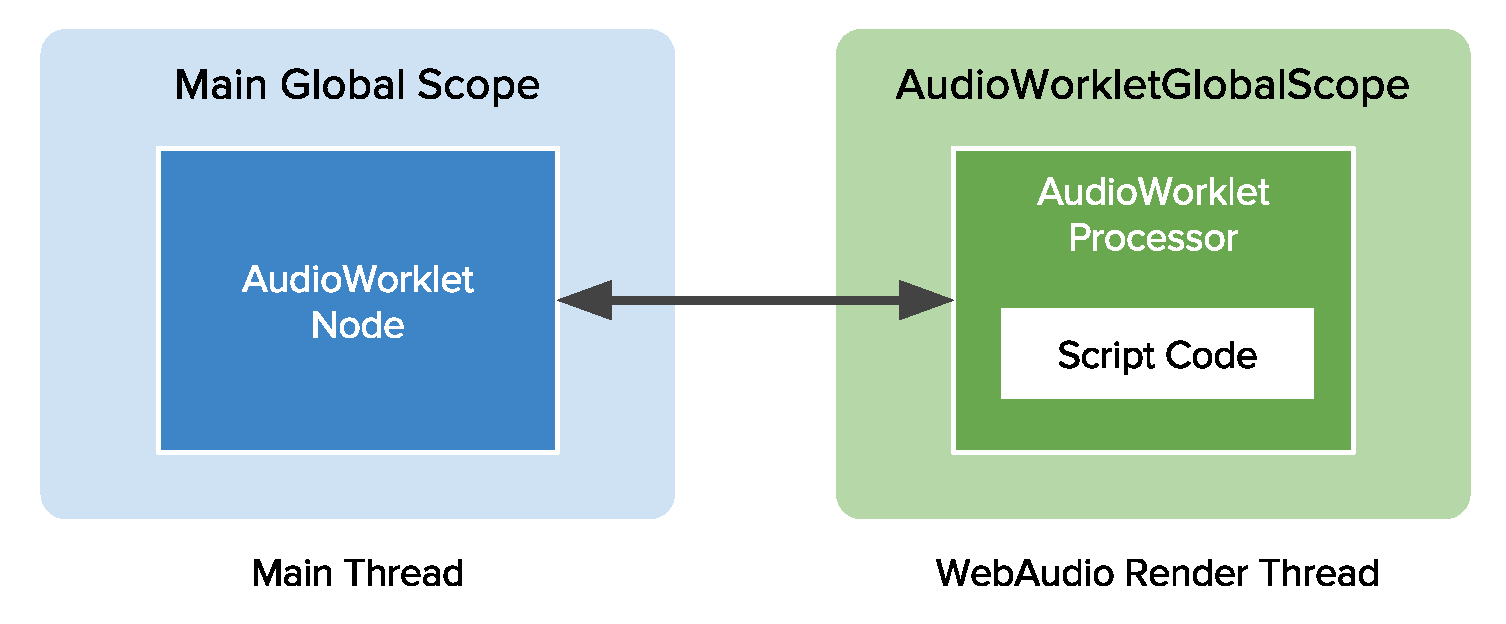
\includegraphics[scale=0.3]{img/webaudio-1.pdf}
   \end{figure}
\begin{itemize}
\item Using AudioWorklet consists of two parts: AudioWorkletProcessor and AudioWorkletNode. 
\item \texttt{AudioWorkletProcessor} represents the actual audio processor written in JavaScript code.
\item \texttt{AudioWorkletNode} takes care of the connection to and from other AudioNodes in the main thread. 
\end{itemize}
\vspace{2 mm}
\center{\tiny{Source: \url{https://developers.google.com/web/updates/2017/12/audio-worklet}}}
\end{frame}
%
\begin{frame}
\frametitle{The Future of Web Audio}
\textit{\scriptsize{``Web-based music software is not free from its fair share of skepticism. The web platform is still fighting an uphill battle to compete with native alternatives and in a large way we are pouring considerable effort into solving problems that are already solved: lower latency, less glitches, multithreaded rendering, and so on. We should be willing to accept the fact that the web platform was not designed for the computer music but be optimistic in our belief that we can change the landscape through gradual progress.''}}\\
\vspace{10 mm}
\tiny{--- Hongchan Choi (2018) \textit{AudioWorklet: The Future of Web Audio}. Proceedings of the International Computer Music Conference.}
%\center{\tiny{Source: Hongchan Choi (2018) AudioWorklet: The future of web audio. Proceedings of the International Computer Music Conference.}}
\end{frame}
%
\begin{frame}
\frametitle{Mini-project development (4/4)}
You are expected to create a mini-project in teams that should be doable within a week. The overall aim is to explore a little bit further Web Audio. Here are different approaches that you can take:
\begin{itemize}
\item Develop an idea based on what we are seeing in class. Feel free to build up everyday, or change if not convinced (from scratch approach).
\item Adapt an existing code to your needs and document what are the changes (remake approach).
\item Combine projects from last week (hybrid approach).
\item Other?
\end{itemize}
\end{frame}
%
\begin{frame}
\frametitle{Working style}
\begin{itemize}
\item Work with the same team throughout the week, ideally across campuses. 
\item Make sure to clarify who has developed what part of the code. For example, divide the work into functions and add the author name at the header of each function.
\item The instructors in both sites will keep an eye on the groups to catch up.
\item There will be 4 time slots during the week to work on the project. 
\item Keep a research journal.
\end{itemize}
\end{frame}
%
\begin{frame}
\frametitle{Assignment 4 Part 3 (10\%) - Final Presentation Mini-Project}
%The order of the groups will be provided by the shuffle algorithm :)
Each group will have 15 minutes (only questions within this time) to explain the following using slides and live demo:
\begin{itemize}
\item \textbf{Description}: What is the title of the project and main concept. Overview of the technologies used.
\item \textbf{Timeline}: Provide an overview of the 3 days that you have been working in the mini-project. What have you been working on?
\item \textbf{Division of labour}: Explain who has been working in what, how you have documented it, working strategies and technologies used.
\item  \textbf{Live demo}: Try to allocate some time for a live demo.
\item \textbf{Achievements}: Give a summary of the achievements of this week through the project. Any progress?
\item \textbf{Challenges}: Give a summary of the challenges that you have been encountering over the week and how you did face them?
\item \textbf{What is next?} e.g. blog post, code repository, website publishing... more development?
\end{itemize}
\end{frame}
%
\begin{frame}
\frametitle{Assignment 5 (10\%) - Written Blog Post Mini-Project 2}
\textbf{Deadline}: February 22, 2019 at 5pm
\begin{itemize}
\item Make sure to include the information requested in your presentation (see previous slide) plus any additional feedback received or follow-up insights.
\item Be familiar with the new metadata to be used so that the blog post has author name, date, the right category (``Audio-Programming''), and a thumbnail for the homepage. See the documentation at: \url{https://github.com/MCT-master/mct-master.github.io/blob/master/README.md}.
\item At least you should use a screenshot and an embedded video showcasing the mini-project. It is a plus if you add links to the source code and a live demo link (e,g. directory in a personal webpage).
\item Add relevant links in the text to generate traffic.
\end{itemize}
\end{frame}
%
\begin{frame}
\frametitle{Final Remarks}
\begin{itemize}
\item \textbf{Post-survey}: please complete by February 22, 2019.
\item \textbf{Web Audio Conference 4-6 December 2019} at NTNU in Trondheim. Participate (music, artworks, demos, talks...)! We will also need student volunteers!
\item Last but not least: \textbf{Congratulations and thank you!} God helg!
\end{itemize}
\end{frame}
%
\begin{frame}
\frametitle{See you at WAC 2019!}
   \begin{figure}
	\includegraphics[scale=0.6]{img/wac2019-header.png}
   \end{figure}
\vspace{10 mm}
\center{\tiny{\url{http://ntnu.edu/wac2019}}}
\end{frame}
%
\begin{frame}
\frametitle{Relevant Links}
\begin{itemize}
\item Syllabus: \url{https://uio.instructure.com/courses/17406/pages/syllabus}
\item GitHub slides \& code: \url{https://github.com/axambo/audio-programming-workshop}
\end{itemize}
\end{frame}
%
%\begin{frame}
%  \frametitle{References}
%  \printbibliography
%\end{frame}
%
\end{document}
